%=========================================================================
% (c) Michal Bidlo, Bohuslav Křena, 2008

\chapter{Úvod}
Diplomová práce se zabývá popisem mobilní a webové aplikace, sloužící pro podporu týmové práce. V úvodní kapitole se věnuji analýze problému a popisu motivace, proč jsem se rozhodl tuto aplikaci vytvořit. Dále analyzuji podobná řešení, zabývající se skupinovou prací. Každé z nich hodnotím podle toho, na kolik je podle mého názoru užitečné a čím se liší od mého řešení. Následuje popis nezbytných poznatků pro základní představu o vývoji mobilní aplikace pro Android a pro detailní pochopení zbytku mojí práce. Dále se zabývám obecnými doporučeními, které se týkají designu a přívětivosti aplikace pro uživatele. Poslední část kapitoly je věnována interakci webové a mobilní aplikace, jaké jsem se rozhodl použít řešení a jaké jsou jiné možnosti.

V kapitole Návrh řešení aplikace NudgeMe informuji o návrhu aplikace. Popisuji a zdůvodňuji zde funkcionalitu, vzhled mé aplikace a také algoritmy, nad kterými aplikace funguje. Také porovnávám a vyhodnocuji různé nápady, které mě v průběhu vývoje napadly a zdůvodňuji také, proč jsem od některých z nich nakonec upustil. 

Dále popisuji testování na koncových uživatelích. Uvádím zde také, jaké existují další možnosti testování s ohledem na Android aplikace. Kapitola se sestává i ze zpětné vazby a jejího zhodnocení. 

V závěru se ohlížím za celou prací, hodnotím její užitečnost, co všechno se stihlo a nestihlo a přikládám představu o tom, jak by se aplikace mohla vyvíjet do budoucna.

\chapter{Analýza problému a motivace pro tvorbu aplikace}

Spolupráce lidí na jednom úkolu není vždy jednoduchá a mnohdy závisí na prostředí, ve kterém je vykonávána. Pravděpodobně je motivace zaměstnanců ve firmě vyšší než studentů u školního projektu. V práci jsou lidé motivováni efektivnějšími prostředky, jako jsou peníze nebo zlepšení pracovního postavení. Ve škole jsou však studenti motivováni známkou z projektu, někdy je práce baví a mnohdy jen chtějí splnit projekt. Dochází tak k častému odkládání projektů nebo špatné informovanosti členů týmu, takže ve výsledku se na projektu pracuje do posledních chvil před odevzdáním a konečný výsledek neodpovídá očekáváním. Pokud členové týmu mohou používat aplikace pro sdílení obsahu, jako jsou např. Google dokumenty, je větší přehled o odvedené práci. Existují však situace a projekty, při kterých tyto nástroje nelze použít, jako jsou manuální práce nebo programování. 

V současné době existuje celá řada programů, které slouží pro řízení a plánování projektů, z nichž některé popisuji v následující kapitole. Obvykle mezi ně patří jednoduché aplikace pro tvorbu seznamu úkolů (To-do lists) nebo robustní aplikace pro velké firmy. Domnívám se však, že s velkými aplikacemi, které jsou mnohdy placené, se nebudou chtít studenti učit pracovat, protože tyto aplikace jsou mnohdy složité a studenti většinu funkcí nevyužijí. Aplikace pro tvorbu seznamů úkolů jsou zase příliš obecné a neprůkazné a není možné porovnat jednotlivé členy podle odvedené práce. 

\section{Motivace pro vytvoření aplikace}

Snahou aplikace je zjednodušit a zefektivnit komunikaci na projektech a zvýšit přehled jednotlivých členů týmu o práci druhých. Aplikace slouží pro posílání reportů jednotlivými uživateli v pravidelných intervalech, kde informují o své provedené práci. Report se sestává z krátkého popisu uživatelovy práce a jejího ohodnocení. Takto vyplněný report je zaznačen do grafu, který znázorňuje intenzitu práce všech členů v čase. Uživatel může využít funkce NudgeMe, díky které odešle krátkou zprávu členům, kteří nezadali report, v níž je vyzývá k jeho zadání. Domnívám se, že hlavní motivací uživatelů spočívá v dosažení co nejlepšího postavení v grafu v rámci týmu. Cílem aplikace je zvýšení aktivity členů týmu porovnáním jejich pracovní výkonnosti s ostatními. Hlavní cílovou skupinou jsou studenti vysokých škol, kteří řeší skupinové projekty. Domnívám se, že díky srovnáním se s ostatními a stručným reportům, může tato aplikace zlepšit efektivitu práce v týmu. Kromě vysokoškoláků a týmů řešících skupinový projekt, mohou aplikaci používat všichni, kteří se chtějí porovnávat s ostatními při provádění nějaké činnosti. Stačí, aby si uživatelé zvolili nějaký společný cíl nebo činnost a do reportů sdělovali svoje úspěchy. 

\chapter{Podobné aplikace pro práci v týmu} \label{apps}

V této kapitole jsou popsány typy aplikací, které úzce souvisí s týmovou prací a komunikací mezi členy týmu. Každá z nich zastupuje jiný přístup řešení dané problematiky. Popisuji je z toho důvodu, abych lépe vysvětlil a odůvodnil vznik svojí aplikace.

\section{Workboard}

Tato aplikace\footnote{Workboard - https://www.workboard.com} je podobná té, kterou vytvářím, ale informování o provedené práci u ní probíhá trošku odlišně. Hlavní položkou je seznam s úkoly, jak je uvedeno na obrázku \ref{work}, který slouží i pro rozdělování práce mezi spolupracovníky. Je možné stanovit určitý cíl projektu, kterého chce uživatel dosáhnout a každý den vyplňovat informace, nakolik se mu povedlo k tomuto cíli přiblížit. Není zde ale možné graficky znázornit výkon celého týmu do jednoho grafu. Také je stanovování cílů spíše bráno jako dodatečná funkcionalita, než jako klíčový ukazatel. Stejně jako moje aplikace umožňuje vyplnit report jen od začátku projektu do aktuálního dne. Jedná se tedy o aplikaci, která se svojí funkcionalitou nachází někde mezi aplikacemi vytvářející seznam úkolů a profesionálním vývojovým softwarem. 

\begin{figure}[H]
\centering
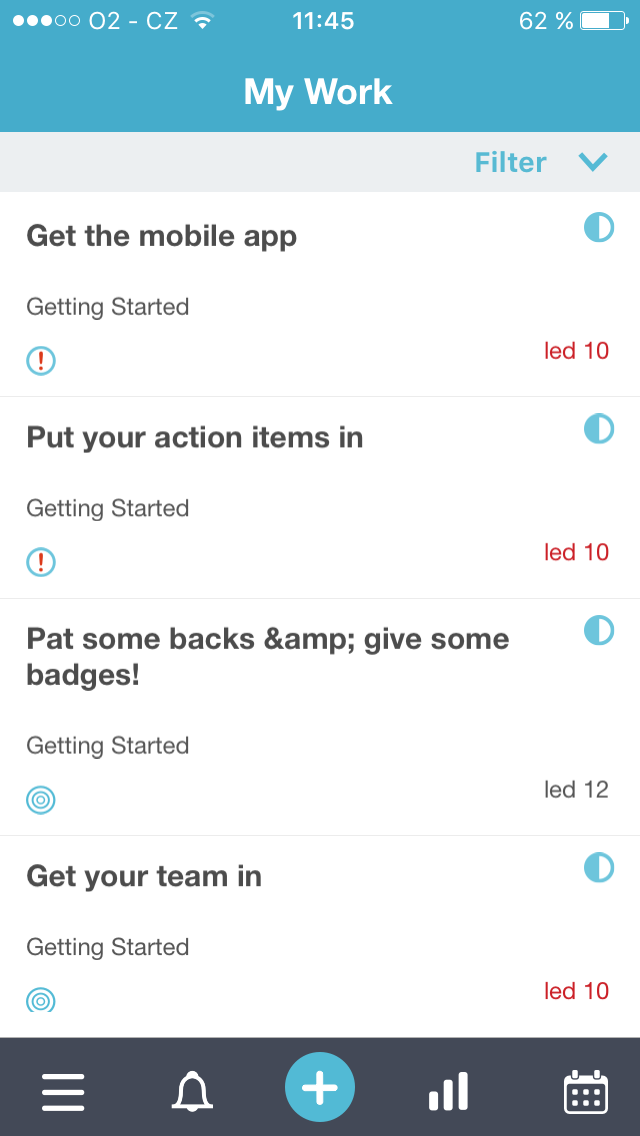
\includegraphics[width= 4cm]{obrazky-figures/IMG_0344}
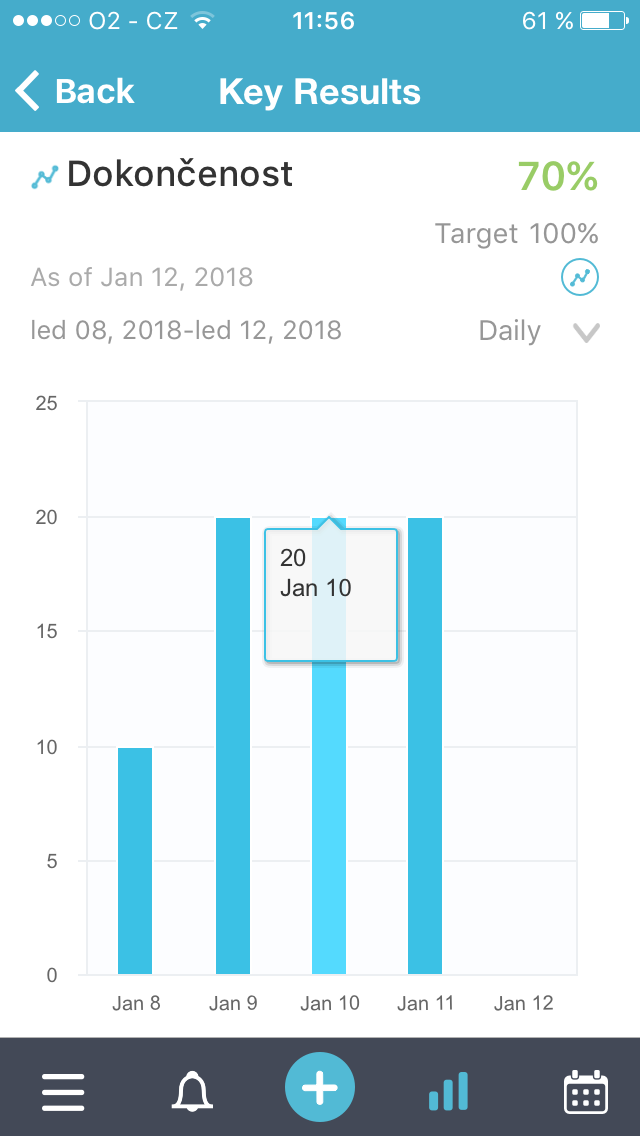
\includegraphics[width= 4cm]{obrazky-figures/IMG_0346}
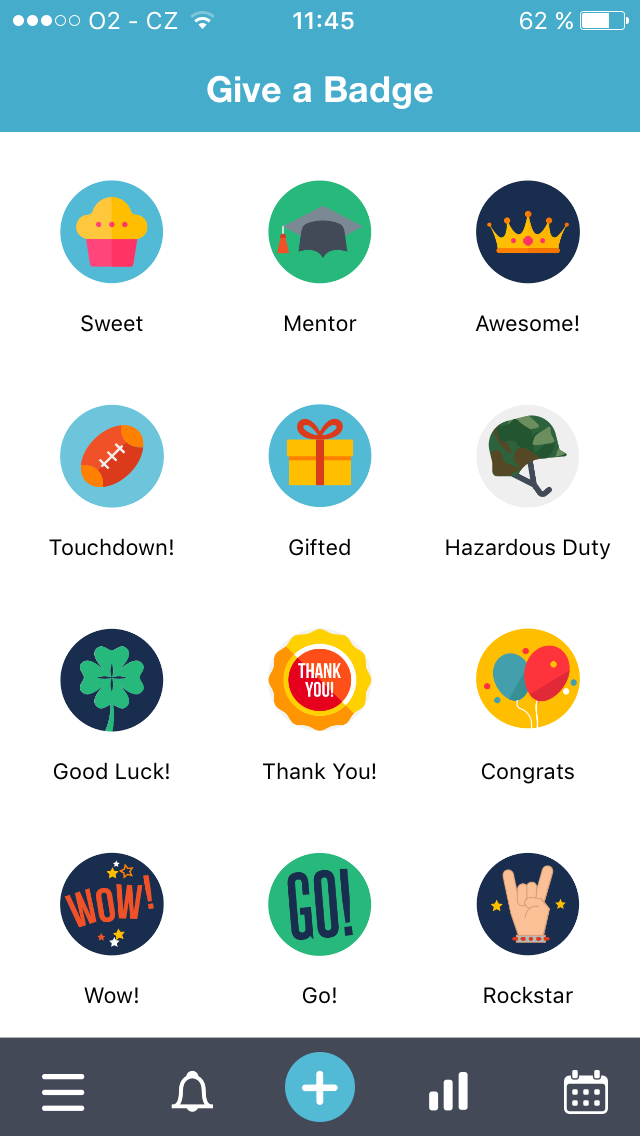
\includegraphics[width= 4cm]{obrazky-figures/IMG_0343}
\caption{Ukázka zobrazuje nejprve seznam úkolů pro konkrétního člena týmu. Dále je zobrazení pokroku na určitém úkolu, kde parametr Dokončenost udává 70\% a sloupcový graf říká, kolik procent práce uživatel udělal v konkrétní den. Za určitou aktivitu je možné udělit ostatním členům týmu odznak, jejichž výčet je na poslední obrazovce. }
\label{work}
\end{figure}

\section{Trello}

\begin{figure}[H]
\centering
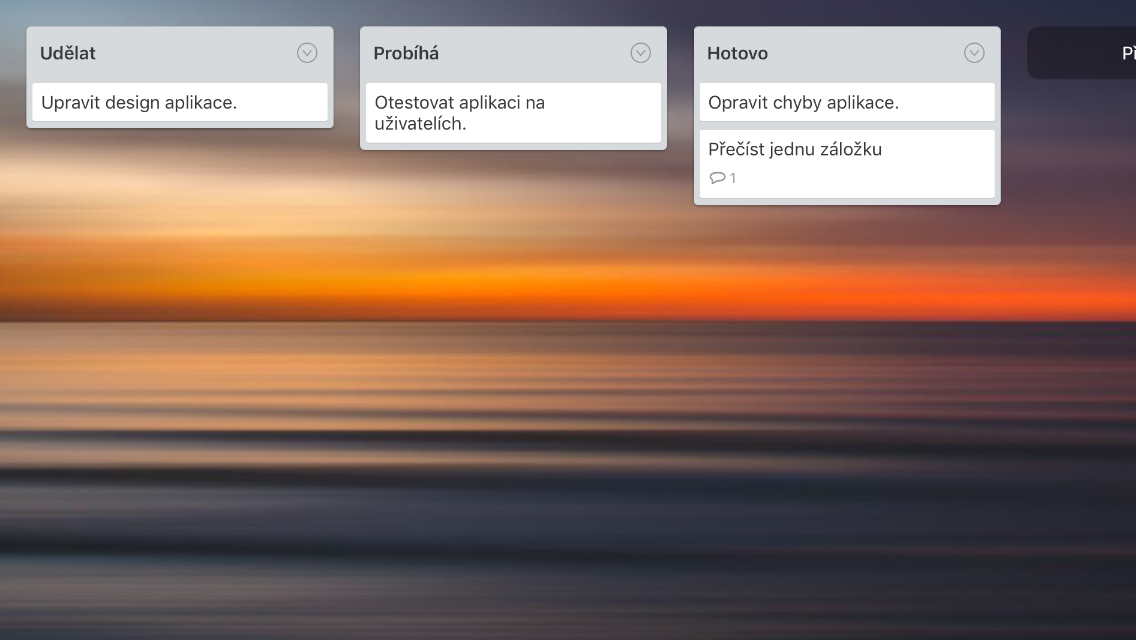
\includegraphics[width= 12cm]{obrazky-figures/IMG_0338}
\caption{Pohled na nástěnku s úkoly a sloupci, popisující určitý stav dokončenosti. Pokud se stav některých úkolů změnil, uživatel jej jednoduše metodou drag \& drop přesune do jiného sloupce.}
\label{trello}
\end{figure}

Další aplikace, kterou jsem se inspiroval, pracuje s kartičkami úkolů a jejich řazením do patřičných sloupců, definujících stav úkolu, podle kterých spolupracovníci poznají, v jaké fázi dokončení se daný úkol nachází. Trello\footnote{Trello - https://trello.com/} jsem zvolil z důvodu jeho velké popularity a také proto, že patří mezi nejjednodušší aplikace používající kartičky pro definování pracovního postupu. Jak je ukázáno na obrázku \ref{trello}, nástěnka je přehledná a dává důraz na co nejrychlejší vytvoření nového úkolu. Při kliknutí na konkrétní úkol se však nabízí více funkcionalit, jako je vložení obrázku, přidání přílohy, hlasování nebo stanovení termínu pro dokončení. 

Inspirací pro moji aplikaci mi byl způsob, jakým mezi sebou jednotliví spolupracovníci komunikují. Při pohledu na nástěnku se dá zjistit, na čem daný člověk pracuje, zda daná práce neměla už být hotová dříve a kolik práce mu ještě zbývá udělat. Z mého pohledu však nenutí uživatele práci rozdělit na menší části, které by dávaly více informací jeho kolegům. Pracovník tedy může mít jednu kartičku s obecným úkolem ve stejné fázi rozpracování i několik dní a ostatní členové nebudou vědět, zda práce probíhá podle plánu nebo se na něčem zasekl. Pro tyto případy je možné přidávat ke kartě komentáře a ptát se uživatele detailněji na na stav jeho práce, avšak tím pro ostatní vyvstává povinnost se aktivně informovat o stavu práce. V případě, že uživatel neprojeví aktivitu a nezeptá se, dozví se, že úkol není splněn až po uplynutí konečného termínu.

\section{Asana}

Jedná se o tzv. aplikaci pro tvorbu seznamu úkolů k provedení. Podobně jako Trello jsou zde vytvářeny úkoly, které mohou být přiřazeny určitému uživateli. Uživatelé konkrétního projektu také mohou vést konverzaci, jak je ukázáno na obrázku \ref{asana}, a posílat si soubory. K dispozici je také nástěnka, která obsahuje graf projektu. Ten informuje o tom, kolik je ke konkrétnímu dni splněno úkolů a kolik jich ještě zbývá.

Asana\footnote{Asana - https://asana.com/} bohužel neumožňuje více specifikovat stav úkolu jinak, než na neuděláno/hotovo, a tím pádem je informovanost členů týmu ještě horší než v případě Trella. Graf stavu práce zase neudává, jestli v průběhu plnění úkolů nenastaly nějaké komplikace, které se mohou znovu objevit.

\begin{figure}[H]
\centering
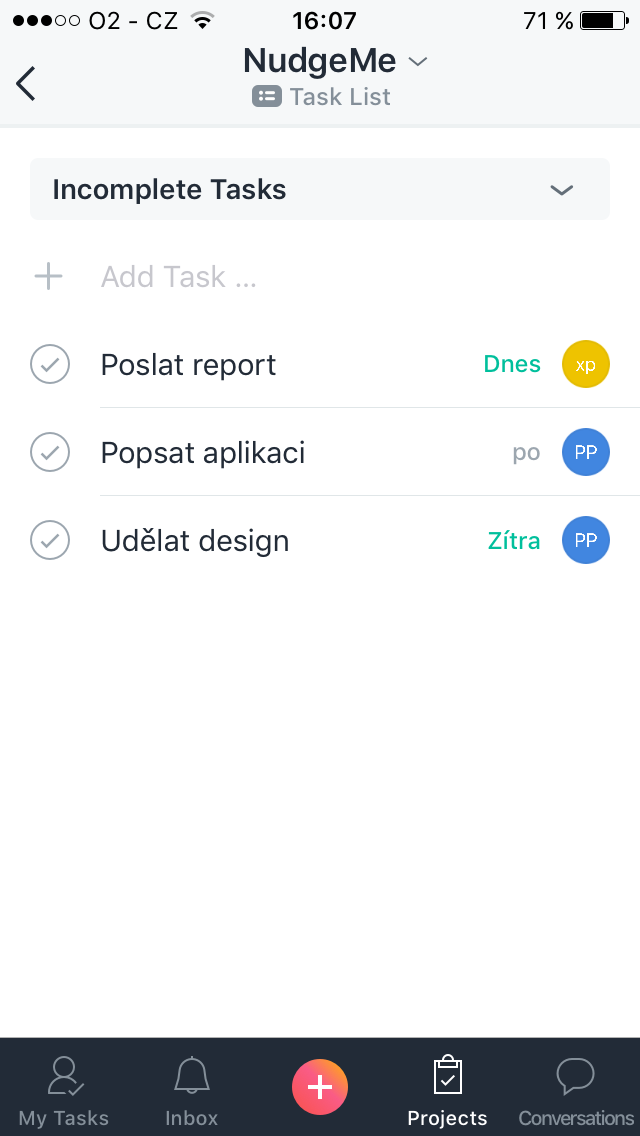
\includegraphics[width= 4cm]{obrazky-figures/IMG_0341}
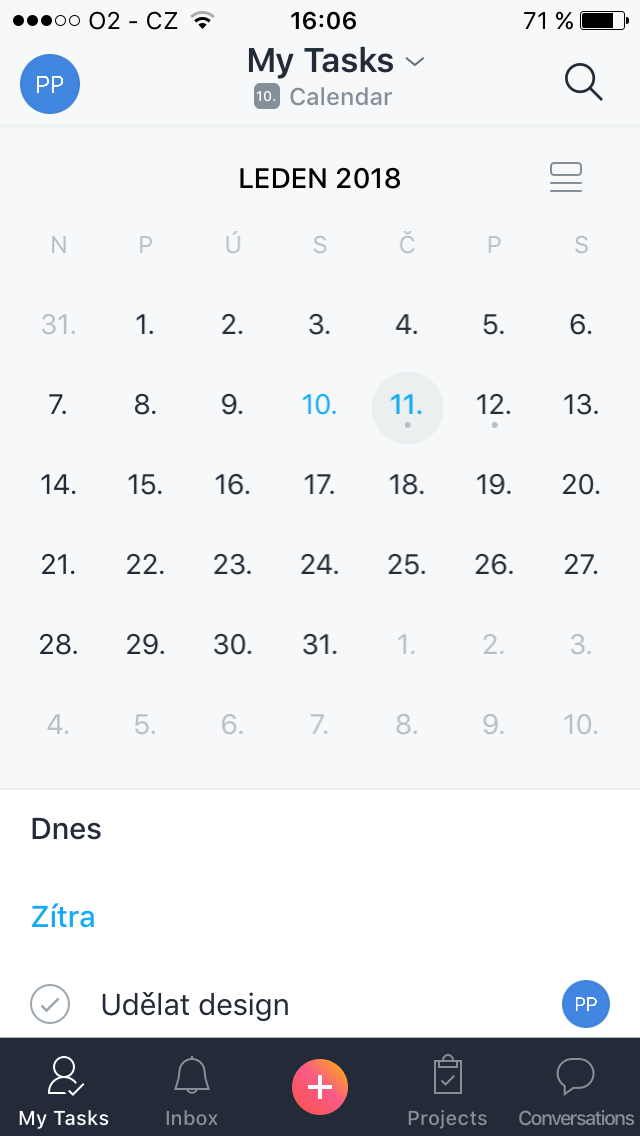
\includegraphics[width= 4cm]{obrazky-figures/IMG_0340}
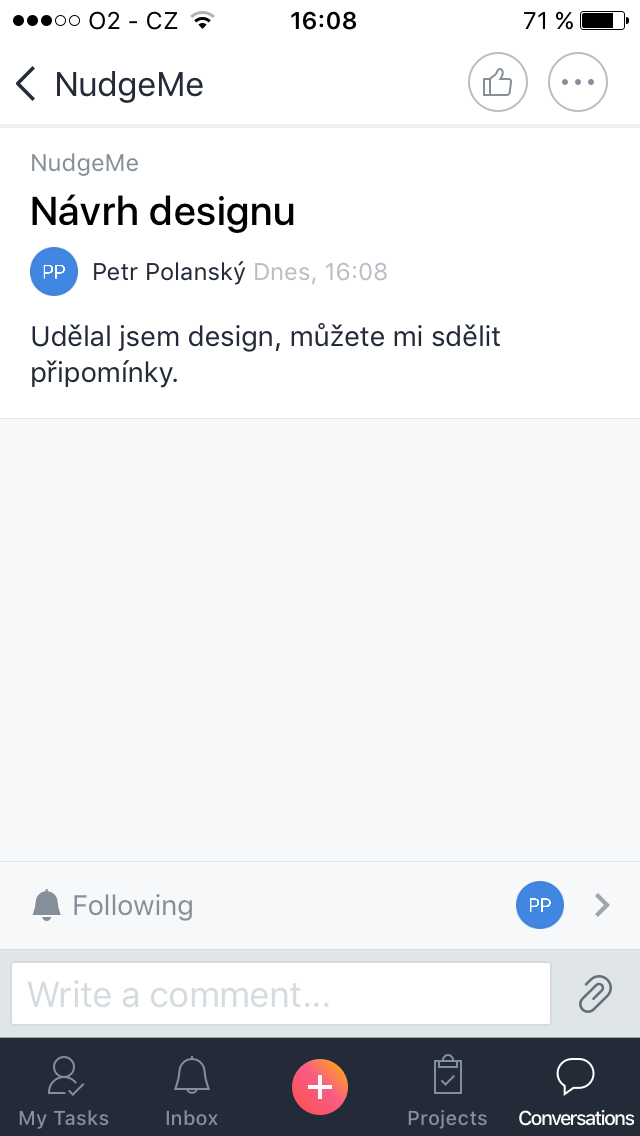
\includegraphics[width= 4cm]{obrazky-figures/IMG_0342}
\caption{Soubor obrázků ukazuje aplikaci Asana a její funkce. Zcela nalevo je obrázek seznamu úkolů, u kterých je ve zkratce uveden vlastník. V kalendáři jsou pak úkoly zaznačeny podle termínů, do kdy mají být dokončeny. Na poslední obrazovce je ukázka posílání zpráv v rámci daného projektu.}
\label{asana}
\end{figure}

\section{Wrike}

Jedná se o program\footnote{Wrike - https://www.wrike.com} sloužící pro profesionální správu a řízení projektů pro větší i menší podniky. Umožňuje plánovat projekt pomocí Ganttova diagramu\footnote{Jedná se o pruhový diagram, který znázorňuje posloupnosti úkolů a jejich závislostí v čase.}, který je ukázán na obrázku \ref{wrike}, nebo diagramu zobrazující vytížení jednotlivých členů týmu. Každý úkol má stanovený začátek a konec a jeho doba trvání je vyobrazena v kalendáři aplikace. Další funkce, jako je vkládání souborů, psaní zpráv a zobrazení nástěnky, jsou podobné jako u Trella a Asany. 

\begin{figure}[H]
\centering
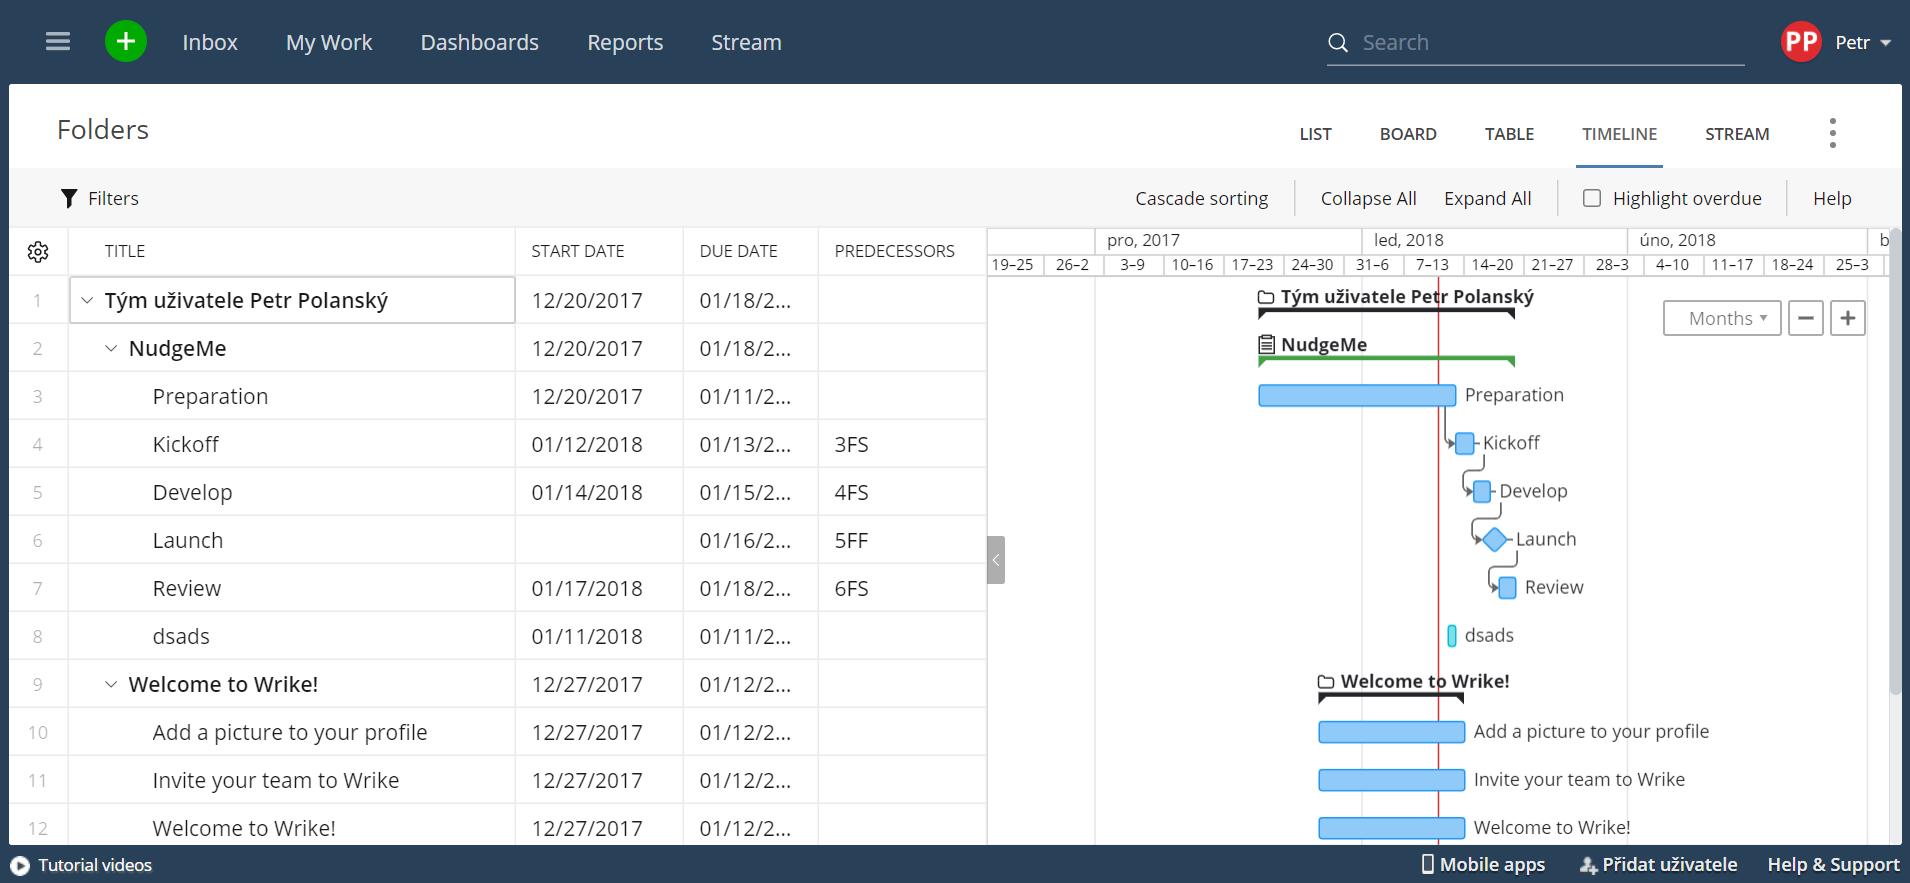
\includegraphics[width= 15cm]{obrazky-figures/Wrike_Gantt}
\caption{Náhled obrazovky pro plánování ve Wrike. Nalevo se nachází seznam jednotlivých úkolů s časovými intervaly pro vykonání. Na pravé straně se nachází Ganttův diagram, který zobrazuje jednotlivé úkoly v pořadí plnění  a jejich závislosti mezi sebou. }
\label{wrike}
\end{figure}

\section{Komunikační aplikace}

Posledním typem aplikací, které slouží pro podporu práce v týmu, jsou aplikace pro psaní zpráv. Mezi nejznámější z nich patří Messenger\footnote{Messenger - https://www.messenger.com} od Facebooku nebo WhatsApp\footnote{WhatsApp - https://www.whatsapp.com}. Obě jsou velmi rozšířené, protože účet na Facebooku má v dnešní době skoro každý a k přístupu na WhatsApp stačí telefonní číslo, které má ještě více lidí. Tyto dvě aplikace ale slouží spíše pro komunikaci mladých lidí a případně pro probírání prací na menších projektech. 

Specializovanější aplikací je pak Slack\footnote{Slack - https://slack.com}, který umožňuje uživateli vytvářet vlastní kanály komunikace, do kterých pouze pozve svoje spolupracovníky. Zároveň umožňuje propojení s některými dalšími aplikacemi jako je Google Drive, Wrike nebo Git.

Tyto aplikace však spíše slouží pro diskuzi a výměnu názorů. Oproti tomu moje aplikace má za cíl sdělit jednoduše a stručně spolupracovníkům, jak je na tom člověk se svými úkoly, které mohly být diskutovány a ustanoveny pomocí výše zmíněných aplikací. 

\chapter{Informace k vývoji pro mobilní systém Android}

V této kapitole popisuji důležité věci, které jsou nutné pro pochopení toho, jak funguje platforma Android, jaké technologie jsem se rozhodl použít, a které poznatky jsou důležité pro přizpůsobení aplikace uživateli. Více jsem rozepsal platformu Firebase, ze které jsem použil její databázi a posílání zpráv. Právě tyto nástroje jsem pak rozvedl do větších podrobností. Podkapitolu o platformě Android jsem převzal z \cite{android}, kromě popisu Android Studia.

\section{Platforma Android}

Jedná se o operační systém, který vytvořila firma Google. V současnosti je systém dostupný pro mobily, tablety nebo chytré hodinky. Android je víceuživatelský linuxový systém, kde každá aplikace vystupuje jako jiný uživatel, má unikátní identifikátor a běží jako vlastní proces, který má svůj vlastní virtuální stroj. Podle příručky pro vývojáře \cite{android} jsou základními stavebními kameny Android aplikace tzv. aplikační komponenty. Každá z nich má jasně stanovenou funkci a životní cyklus. Dělí se na Activities, Services, Broadcast receivers a Content providers. 

\begin{itemize}
\item \textbf{Activities} \,---\, slouží pro interakci s uživatelem, každá z nich představuje jedno okno aplikace s definovaným rozhraním, mohou spustit jinou aktivitu, která si uchovává informace o předešlé pro případ, že by se na ni chtěl uživatel vrátit,
\item \textbf{Services} \,---\, zajišťují běh procesů na pozadí aplikace,
\item \textbf{Broadcast receivers} \,---\, zajišťují doručení událostí, které mohou být doručeny i v případě, že aplikace neběží,
\item \textbf{Content providers} \,---\, slouží pro řízení a sdílení aplikačních dat s možností je uložit do souborů nebo databází.
\end{itemize}

Activities, Services a Broadcast receivers je možné aktivovat asynchronní zprávou zvanou Intent. Android funguje na principu nejnižších privilegií, kde každá aplikace má přístup jen k těm zdrojům, které potřebuje. Existují však mechanismy, kdy aplikace může sdílet informace s jinou aplikací. Pro instalaci aplikace na zařízení slouží soubor APK\footnote{APK - Android Package Kit}, který je vytvořen zkompilováním zdrojových kódů a ostatních souborů, jako jsou aplikační zdroje (resources). Ty slouží pro vizuální prezentaci aplikace. Pomocí XML souborů, které jsou odděleny od zdrojových kódů, může uživatel definovat styly, barvy nebo animace pro svoji aplikaci. Každý tento zdroj má přiřazen unikátní identifikátor, přes který je možné se na zdroj odkazovat v kódu.

\subsection*{Android Manifest}

Jedná se o soubor, který slouží pro specifikování práv pro aplikaci, API\footnote{API - Application Programming Interface} knihoven nebo  hardwaru a softwaru, který může aplikace využívat (kamera, bluetooth). Dále se mohou specifikovat požadavky na zařízení a jeho zdroje, aby bylo zaručeno, že aplikace bude fungovat. To slouží např. při znemožnění stažení aplikace z Google Play, pokud zařízení nemá vyhovující prostředky pro běh aplikace. Pokud chce uživatel využívat výše zmíněné aplikační komponenty, musí je v tomto souboru také uvést.
 
\subsection*{Popis vrstev architektury platformy Android}

Následuje popis jednotlivých vrstev Android architektury, jejichž závislosti jsou ukázány na obrázku \ref{archi}, který je převrat z \cite{android}.

\begin{figure}[t]
\centering
\includegraphics[width= 5cm]{obrazky-figures/architecture}
\caption{Diagram architektury platformy Android. Vrstvy postupují od nejvyšší, což jsou Systémové aplikace, až po tu nejnižší, kterou je Linuxové jádro.}
\label{archi}
\end{figure}

\begin{itemize}
\item Linuxové jádro \,---\, poskytuje prostředky vyšším vrstvám a slouží pro správu nižších prostředků, jako je baterie nebo zabezpečení aplikace,
\item Hardwarová abstrakční vrstva \,---\, se sestává z modulů knihoven a poskytuje rozhraní pro práci s hardwarovými komponentami, když o ně API požádá,
\item Android Runtime \,---\, v rámci každé aplikace běží Android Runtime, který poskytuje několik užitečných funkcí, jako je např. optimalizovaný garbage collection,
\item Nativní C/C++ knihovny \,---\, poskytují podporu např. vysoce náročným procesům 2D a 3D grafiky,
\item Java API framework \,---\, zahrnují content providers a manažery, kteří spravují např. zdroje, notifikace nebo aktivity,
\item Systémové aplikace \,---\, jedná se o aplikace, které jsou k dispozici v zařízení už po instalaci a uživatel k nim může přes svoji aplikaci přistupovat (kamera, kalendář, bluetooth, ...).
\end{itemize}

\subsection*{Android Studio}
Jedná se o IDE\footnote{IDE - Integrated Development Environment} vytvořené firmou Google pro programování aplikací pro platformu Android. Jednou z hlavních předností tohoto prostředí je zabudovaný emulátor mobilních zařízení. Vývojář si může vybrat mezi různými typy zařízení i verzí operačního systému. Nahrávání aplikace do emulátoru je jednoduché a v případě menší změny se aplikace nemusí ani restartovat. Tímto způsobem testování může uživatel dopředu zjistit, jak se jeho aplikace přizpůsobuje určitému rozměru úhlopříčky displaye. 

\begin{figure}
\centering
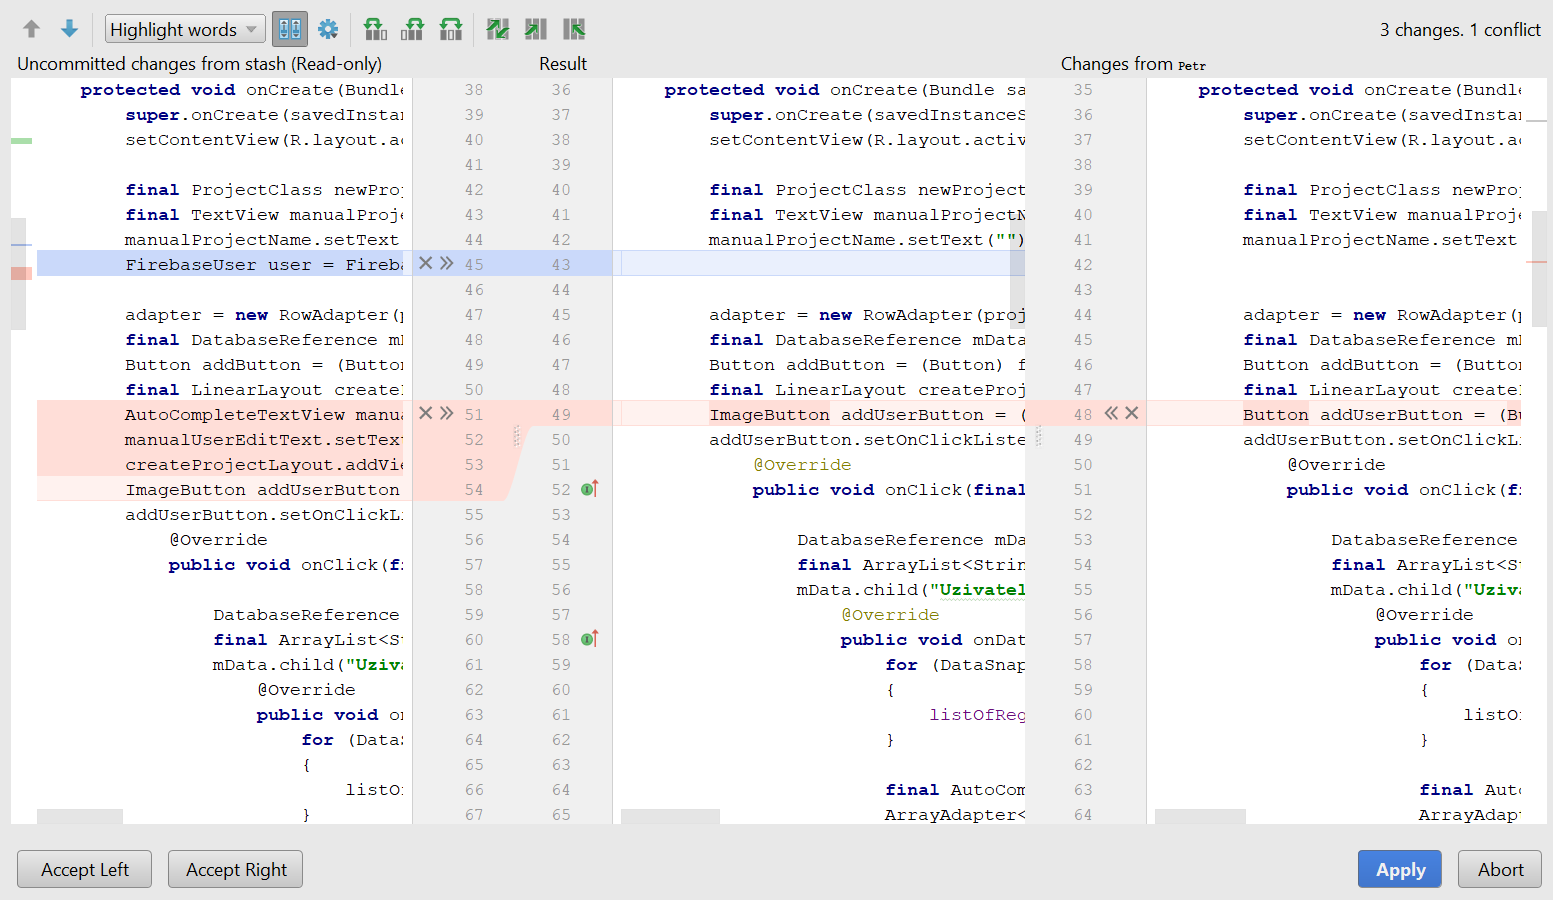
\includegraphics[width= 15cm]{obrazky-figures/resolving_conflicts1}
\caption{Nástin řešení konfliktů v Android Studiu. Situace nastává, když uživatel přepíná mezi větvemi při používání Gitu. Na obrázku je vyobrazen konflikt mezi změnami, na které ještě nebyl spuštěn commit, a větví s názvem Petr.}
\label{resolv}
\end{figure}

Pro podporu tvorby kódu ve více lidech je k dispozici Git. Je vhodný zejména při obecných úkonech, jako je stažení repozitáře a poslání změn na server. Při řešení případných konfliktů lze použít porovnání jednotlivých souborů za pomoci GUI, které je ukázáno na obrázku \ref{resolv}, kde uživatel vybere, které změny z jakého souboru chce ponechat ve finální verzi. Jedna z doplňujících funkcí je možnost kontroly a odstranění referencí na knihovny, které jsou vloženy v kódu, ale v aplikaci nejsou využity. Uživatel díky GUI může přepínat mezi více větvemi nebo porovnávat stejné soubory na různých větvích.

Studio používá pro sestavení aplikace nástroj Gradle\footnote{Gradle - https://gradle.org}, který zajišťuje jednoduchý import knihoven. Díky tomu dochází k snadnému propojení s knihovnou Firebase. Další užitečnou funkcí je Vector asset sloužící k vložení a převodu vektorových obrázků na zdrojový soubor XML. Jsou k dispozici ikony material designu, který popisuji dále v této kapitole.  

\section{Firebase}

Jedná se o API, které slouží pro podporu vývoje jak mobilních, tak i webových aplikací. Původní firma byla koupena Googlem a díky tomu Firebase snáze spolupracuje s ostatními Google funkcemi a nástroji, jako je např. Android Studio. Vývoj je také umožněn pro iOS a Unity.

\begin{table}
\centering
    \begin{tabular}{| l | l |}
    \hline
    Název technologie & Popis \\ \hline
    Analytics & sledování výkonnosti a používání aplikace \\ \hline
  	Authentication & přihlášení přes email, Facebook, Git atd. \\ \hline
    Test lab & testování aplikace na zařízeních v datovém centru Googlu \\ \hline
    Remote Config & změnění aplikace bez nutnosti vytváření aktualizace \\ \hline
    AdMob & řešení pro vložení reklamy do aplikace \\ \hline
    Cloud Firestone & alternativa k databázi pracující v reálném čase. \\ \hline   
    \end{tabular}
    \caption{Výčet některých užitečných funkcí, které nabízí Firebase. }
    \label{table}
\end{table}

Ve své aplikaci jsem použil databázi pracující v reálném čase, funkce pro autentizaci a posílání zpráv přes cloud. Všechny tyto technologie jsem si dovolil popsat v následujících podkapitolách. Tabulka \ref{table} ve stručnosti popisuje další užitečné funkce Firebase, které jsou pak detailněji popsány v příslušné dokumentaci \cite{firebase}.

\subsection*{Databáze pracující v reálném čase}
Jedna z hlavních funkcí Firebase je poskytování databáze, která pracuje skoro v reálném čase. Data nejsou uspořádána relačně, ale do JSON struktur a jsou k dispozici na všech zařízeních, na které se uživatel přihlásí. Pro čtení a zápis dat existují speciální funkce. Pokud uživatel chce číst z databáze, musí nastavit tzv. poslouchače (listener) na určitou část z databáze. Poslouchač poté uživateli předá tuto část i se všemi zanořenými daty. Předání je spuštěno určitou událostí, např. změnou části databáze nebo modifikováním synovského elementu. Poslední možností je vyvolání dat bez čekání na událost. V takovém případě však nejsou informace dostupné okamžitě, ale s menším zpožděním. Doporučuje se proto, jakoukoliv práci se získanými daty provádět uvnitř funkce pro čtení. Program totiž nečeká na to, až data dorazí, ale přejde ihned na další řádek kódu. Může se stát, že program bude chtít pracovat s daty, která však ještě nejsou k dispozici. Databázi lze také upravovat ručně přes Firebase konzoli\footnote{Firebase konzole -  https://console.firebase.google.com/}.   

Databáze taktéž umožňuje práci v offline režimu, když není dostupné internetové připojení. Firebase pak pracuje pouze s daty, která jsou uložena v pomocné paměti (cache). V případě provádění dotazů nad databází jsou tyto příkazy uloženy a po obnovení internetového připojení provedeny ve stejném pořadí, v jakém byly zadány.

\subsection*{Autentizace}
Možnost přihlášení a registrace uživatelů je velice snadná, protože je zapouzdřena do několika knihovních funkcí. Ty přijímají jako parametry uživatelův email a heslo. Voláním funkce pro registraci s údaji, které už v databázi existují, lze ověřit, zda daný uživatel už je registrován. Kromě přihlašování a registrace přes email jsou rovněž implementovány funkce pro přístup pomocí účtu na Facebooku, Twitteru, GitHubu nebo Googlu.

\subsection*{Posílání a přijímání zpráv přes cloud}

Firebase umožňuje přes cloud posílat zprávy na konkrétní zařízení. Samotné posílání je možné několika způsoby. Základní dělení spočívá v tom, zda má být zpráva poslána jednotlivci nebo skupině. Pro poslání zprávy jednotlivci je třeba jako klíč "to"~ uvést speciální token příjemce, který se získá funkcí \texttt{FirebaseInstanceId.getInstance().getToken()}. Posílání zpráv na více zařízení se dělí na dva způsoby. Zařízení může být registrováno k odběru určitého tématu (topic) a tedy každá zpráva s tímto označením bude doručena všem odběratelům. Každé zařízení pak může být registrováno pro více témat. Druhý způsob je posílání zpráv určité skupině zařízení. Uživatel ve zprávě definuje skupinu zařízení a pošle tuto zprávu serveru. Ten jako odpověď pošle notifikační klíč dané skupiny. Zařízení se do této skupiny přihlásí právě prostřednictvím daného klíče a unikátního identifikátoru, který si uživatel zvolí. Rozdíly mezi strukturami zpráv\footnote{Uvedené struktury JSON formátu jsou upraveny z https://firebase.google.com/docs/cloud-messaging/send-message} pro jedno zařízení resp. pro odběr tématu jsou ukázány na listingu \ref{lst:jeden} resp. \ref{lst:topic}.

\lstset{
    string=[s]{"}{"},
    stringstyle=\color{blue},
    comment=[l]{:},
    commentstyle=\color{black},
}

\begin{lstlisting}[frame=single, caption={Příklad struktury zprávy pro poslání konkrétnímu uživateli. Na prvním řádku je adresa serveru, druhý udává formát zprávy a na třetím je autorizační klíč, který je unikátní pro každou aplikaci ve Firebase a odlišuje tak zprávy jiných aplikací. Klíč "to"~ obsahuje token příjemce.}, captionpos=b, label={lst:jeden}]
https://fcm.googleapis.com/fcm/send
Content-Type:application/json
Authorization:key=AIzaSyZ-1u...0GBYzPu7Udno5aA

{ "to" : "bk3RNwTe3H0:CI2k_HHwgIpoDKCIZvvDMExUdFQ3P1...",
  "data" : {
    	"message": "Zprava pro konkretniho uzivatele."
  }  
}

\end{lstlisting}

\begin{lstlisting}[frame=single, caption={Příklad struktury zprávy pro poslání na konkrétní téma.}, captionpos=b,label={lst:topic}]
https://fcm.googleapis.com/fcm/send
Content-Type:application/json
Authorization:key=AIzaSyZ-1u...0GBYzPu7Udno5aA

{ "to": "/topics/nas_projekt",
  "data": {
    	"message": "Posilam tento dulezity text.",
   }
}
\end{lstlisting}

V reakci na odeslanou zprávu server pošle odpověď, zda byla zpráva úspěšně doručena. Odpověď se liší podle způsobu odeslání. Pokud byla zpráva odeslána pro určité téma, v případě úspěchu odpověď obsahuje identifikátor dané zprávy. Jestliže odeslání nebylo úspěšné, zpráva bude obsahovat chybovou hlášku, informující o důvodu nezdaru. Mezi důvody může patřit špatně zadaný token při posílání na konkrétní zařízení, nesprávně definovaný formát JSON struktury zprávy nebo špatně zadaný parametr zprávy. Pro posílání zprávy skupině zařízení následuje odpověď, která udává, na kolika z nich byla zpráva úspěšně přijata a na kolika nikoliv.

Pro přijímání zpráv je nutné přepsat metodu \texttt{OnMessageReceived()}, v jejímž parametru \textbf{remoteMessage}  je obsažena přijatá zpráva. 

\subsection*{Material Design}

\begin{figure}[H]
\centering
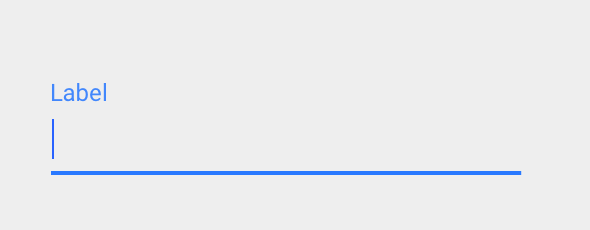
\includegraphics[width= 5cm]{obrazky-figures/label1}
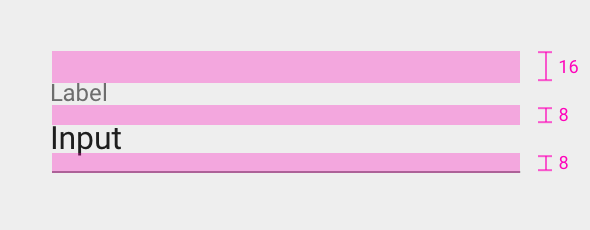
\includegraphics[width= 5cm]{obrazky-figures/label}
\caption{Příklad Material designu pro přesné zvolení koordinace řádku s textem a nadpisem.}
\label{label}
\end{figure}

Jedná se o soupis poznatků a návrhů pro vytvoření jednotného a přehledného grafického rozhraní mobilní aplikace. Postupně se začlenil do všech zařízení, které mají operační systém Android (tablety, Chromebooky). Dalo by se říci, že se jedná o uživatelskou příručku \cite{material}, která popisuje, jak správně tvořit design jednotlivých komponent, např. menu, layout, textový box, tak i doporučení, kdy je vhodné použít kterou komponentu. Na obrázku \ref{label} je ukázáno, jaké jsou například doporučovány rozestupy mezi textovým polem a jeho nadpisem. Jak je vidět, je mezi nimi rozestup 8dp\footnote{dp - density-independent pixels. Doporučuje se tato jednotka používat pro rovnoměrné zobrazení elementů při různých hustotách obrazovek. Obrázky jsou převzaty z https://material.io/guidelines/components/text-fields.html\#text-fields-layout.}. Na obrázku \ref{desc} je zase příklad uzpůsobení popisků pro co nejlepší informovanost uživatele. 

\begin{figure}[H]
\centering
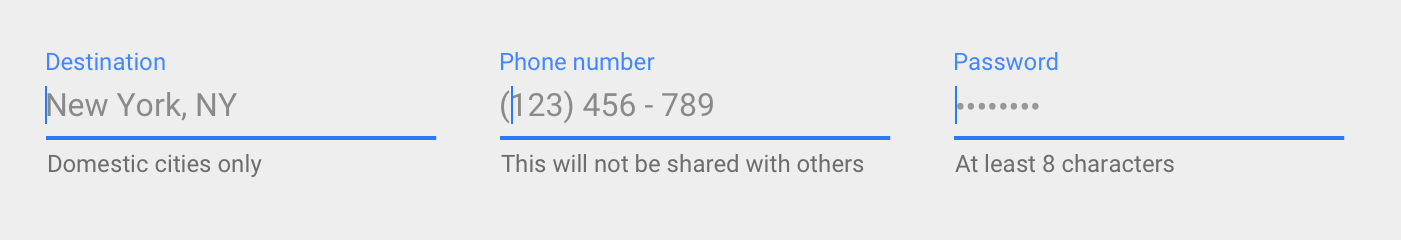
\includegraphics[width= 11cm]{obrazky-figures/description}
\caption{Náhled na řádky textu, které se skládají ze dvou popisků. Horní nadpis udává, co má uživatel vyplnit a dolní popisek sděluje další informace, které by měl uživatel vědět.}
\label{desc}
\end{figure}

\section{Poznatky o tvorbě designu aplikací}

\begin{figure}[H]
\centering
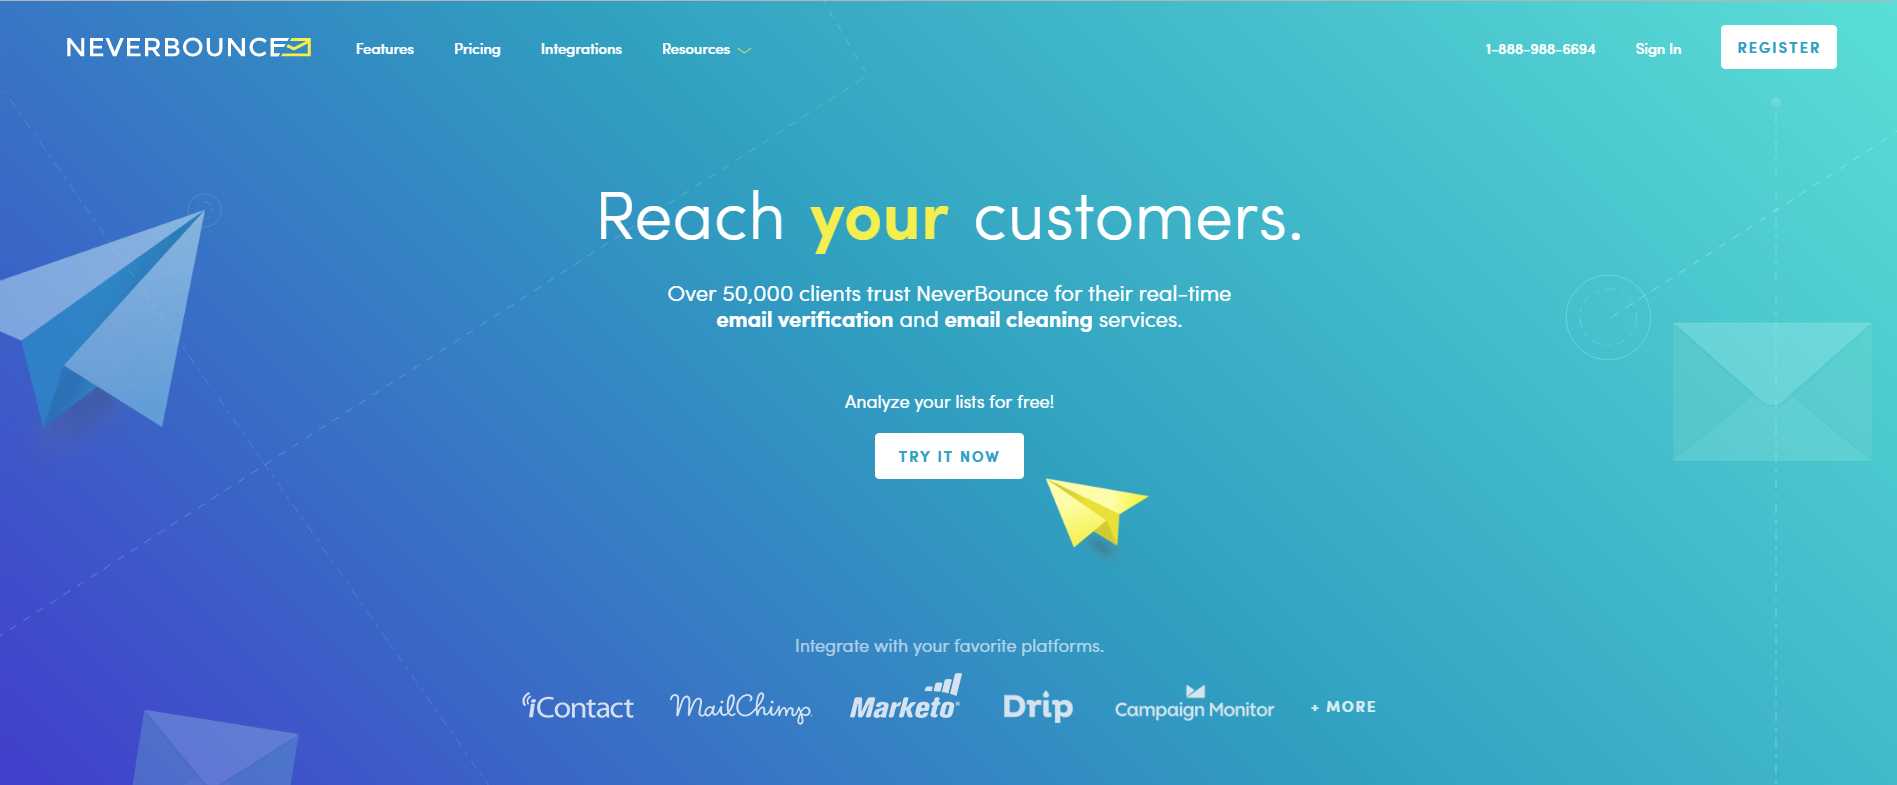
\includegraphics[width= 15cm]{obrazky-figures/good_design}
\caption{Příklad webové stránky, která má pěkný a přehledný design. Uprostřed je stručně popsáno, o čem tato stránka je a co má udělat. Menu je situováno na kraj, aby neodvádělo pozornost od hlavní funkce stránky.}
\label{good}
\end{figure}

Kromě toho, že aplikace musí splňovat veškeré funkce, které si vývojář vysnil, musí se také líbit zákazníkům. Existuje spousta aplikací, které jsou stejně dobré nebo i lepší, ale uživatel si zvolí tu, která má lepší design, je přehlednější a obecně snadnější na ovládání. Tyto principy je třeba ctít jak při vývoji webových, tak i mobilních aplikací. Při vytváření vzhledu aplikace je třeba brát v potaz i psychologii a myšlení uživatele. Důležitý je první kontakt s aplikací, který z větší části rozhodne o tom, zda si uživatel zvolí právě tento program. Steve Krug ve své knize \cite{Krug} upozorňuje na to, jak důležité je udělat aplikaci přehlednou a co nejjednodušší. Uživatelé nechtějí přemýšlet a při jakékoliv práci navíc ztrácejí o aplikaci zájem. Důležité je také brát v potaz rozmístění prvků na obrazovce. Podle článku o vlivu psychologie na design \cite{Than} uživatelé lépe reagují na aplikace, které jsou navrženy podle určitého vzoru/rozestavení, se kterým se již v minulosti  setkali a tedy se v aplikaci lépe orientují. Když už uživatel aplikaci najde, v několika málo okamžicích se rozhoduje o tom, zda pro něj má přínos, nebo jestli se k ní ještě někdy vrátí. Jak docílit toho, aby se zákazník rozhodl aplikaci využít a aby tato dostatečně upoutala pozornost, popisuje Alexander Dawson ve své knize \cite{Dawson}. Také udává, že je dobré se inspirovat aplikacemi, které svým osobitým designem získaly velkou oblibu mezi lidmi. Na obrázku \ref{good} je příklad dobře navržené a přehledné stránky\footnote{Obrázek stránky byl převzat od společnosti NeverBounce - https://neverbounce.com/.}.

\section{Interakce webové a mobilní aplikace}

Pro snadnou spolupráci mezi webovou a mobilní aplikací jsem zvolil platformu Firebase. Vyhovuje totiž přesně požadavkům, které pro svoji aplikaci vyžaduji. Její databáze umožňuje aktualizaci dat při jakékoliv změně, podporuje vývoj jak pro mobilní zařízení, tak i pro webové aplikace a nabízí spoustu užitečných funkcí, jako je ukládání dat do cloudu, posílání zpráv přes cloud a nástroje pro testování. Pro implementaci komunikace je v rámci vývoje webové aplikace použit Javascript. Je také umožněno backend implementovat pomocí Node.js.

Jako jedna z alternativ se nabízí Amazon AWS\footnote{Amazon Web Services - https://aws.amazon.com/mobile}, který disponuje podobnými funkcemi. Firebase se mi však zdála vhodnější pro malou a jednoduchou aplikaci. Dále se nabízí Realm\footnote{Realm - https://realm.io}, který oproti Firebase umožňuje mít lokální databázi v mobilu.

\chapter{Návrh aplikace NudgeMe}

Kapitola se věnuje důkladnému popsání funkcionality, návrhu a interakce aplikace s uživatelem. Vše je popsáno pro mobilní aplikaci, která poskytuje veškerou funkcionalitu, oproti webové aplikaci. Ta slouží pouze pro přehlednější zobrazení uživatelových projektů a jejich částečnou analýzu. Nakonec následuje popis struktury databáze.

\section{Popis funkcionality}

Každý uživatel když aplikaci spustí, tak prvně uvidí graf, znázorňující výkonnost jednotlivých členů týmu v čase. Ihned tedy bude vědět, v jaké situaci se nachází on a jeho kolegové. Cílem je uživatele, pomocí srovnávání s ostatními, vybudit k větší aktivitě na projektu. Jednoduchost aplikace má také za cíl, aby se ji uživatelé nebáli používat a vraceli se k ní pravidelně. Poslání reportu je velmi rychlé a ihned poté je jeho hodnota zanesena do grafu. Obrázek \ref{use_case} ukazuje, jaké funkce aplikace podporuje.  

\begin{figure}[H]
\centering
\includegraphics[width= 7cm]{Use_case}
\caption{Use case diagram, který popisuje hlavní funkce aplikace, které může uživatel použít. Kromě nich je také umožněno spravovat uživatelův profil, přidat nebo odebrat členy projektu nebo přepínat mezi uživatelovými projekty. }
\label{use_case}
\end{figure}
 
Po uživatelově úspěšném přihlášení se zobrazí hlavní obrazovka \ref{fig:hlavni}. Graf na obrazovce patří k aktuálně vybranému projektu. Jsou na něm vyznačeni všichni spolupracovníci, kteří se daném projektu podílejí. Algoritmus vykreslování zadaných hodnot do grafu pracuje s intervalem (-1,1) na y ose. Při zadávání pozitivních hodnocení se křivka blíží k 1 a při negativních k -1. Zadáním neutrálního výrazu se křivka blíží k 0. Graf je v jistých ohledech interaktivní a umožňuje přiblížení, resp. oddálení nebo posun doleva, čímž se zobrazí hodnoty reportů z dřívějšího období. Oproti tomuto návrhu je křivka každého člena stejné barvy, jako jsou obrázky jejich avatarů v horní polovině okna. Ty jsou částečně inspirovány aplikací Messenger, kde však slouží pro zobrazení konverzace s dotyčným uživatelem. Pomocí menu uživatel může přepínat mezi svými projekty. Historie návrhu menu je zobrazena na obrázku \ref{fig:menus}. Konečná verze je inspirována přepínáním mezi kanály v aplikaci Slack. 

Tlačítko NudgeMe na hlavní obrazovce \ref{fig:hlavni} slouží pro poslání zprávy všem uživatelům, kteří v aktuální den nezadali svůj report. V reakci na zprávu se uživateli zobrazí notifikace, která umožní, po kliknutí na ni, přejít ihned na obrazovku \ref{fig:report} pro vyplnění reportu. Upozornění přijde na každé zařízení, na kterém je uživatel aktuálně přihlášen. V případě, že již má určitý uživatel vyplněn report na tento den a někdo jiný pošle zprávu, nebude uživateli, který report vyplnil, zobrazena tato notifikace. Tento princip slouží pro pobízení spolupracovníků ke sdělení informací o provedené práci. Jedná se o podobnou funkci, jako je "šťouchnutí"~ přátel na Facebooku.

\begin{figure}[H]
    \centering
    \begin{subfigure}[b]{0.2\textwidth}
        \includegraphics[width=\textwidth]{obrazky-figures/Screen_graph}
        \caption{}
        \label{fig:hlavni}
    \end{subfigure}
    \begin{subfigure}[b]{0.2\textwidth}
        \includegraphics[width=\textwidth]{obrazky-figures/Screen_reports}
        \caption{}
        \label{fig:reporty}
    \end{subfigure}
    \begin{subfigure}[b]{0.2\textwidth}
        \includegraphics[width=\textwidth]{obrazky-figures/Screen_projects}
        \caption{}
        \label{fig:projekty}
    \end{subfigure}
    \begin{subfigure}[b]{0.2\textwidth}
        \includegraphics[width=\textwidth]{obrazky-figures/Screen_report}
        \caption{}
        \label{fig:report}
    \end{subfigure}
    \caption{Návrh hlavních obrazovek aplikace. Na hlavní obrazovce \ref{fig:hlavni} je vyobrazen graf, obrázky avatarů všech členů projektu a tlačítka pro přechod na obrazovku \ref{fig:report} a pro poslání NudgeMe. Na dalším snímku \ref{fig:reporty} je výpis reportů uživatele, kde je dále uvedeno jeho jméno a příslušný avatar. Snímek \ref{fig:projekty} zobrazuje projekty, kde u každého z nich se nachází jeho název a avataři příslušných členů. Po kliknutí na konkrétní projekt se zobrazí jeho podrobnější informace. Navíc je k dispozici tlačítko pro přidání nového projektu. Nakonec je snímek \ref{fig:report} pro vyplnění reportu.}
    \label{fig:dulezite}
\end{figure}

Obrazovka \ref{fig:report} zobrazuje, co všechno je součástí reportu. Nejprve je to datum, které je primárně nastaveno na aktuální, dále textový blok pro napsání krátké zprávy informující ostatní o provedené práci a výběr smajlíka symbolizující pocit z odvedené práce. Pokud se stane, že uživatel v předchozích dnech nevyplnil reporty, po odeslání reportu na aktuální den se automaticky dogenerují reporty do databáze pro nevyplněné dny a budou obsahovat speciální hodnoty, které je odliší od zadaných reportů. 
 
\begin{figure}[H]
    \centering
    \begin{subfigure}[b]{0.2\textwidth}
        \includegraphics[width=\textwidth]{obrazky-figures/Screen_without_menu}
        \caption{}
        \label{fig:without_menu}
    \end{subfigure}
    \begin{subfigure}[b]{0.2\textwidth}
        \includegraphics[width=\textwidth]{obrazky-figures/Screen_with_menu}
        \caption{}
        \label{fig:with_menu}
    \end{subfigure}
    \begin{subfigure}[b]{0.2\textwidth}
        \includegraphics[width=\textwidth]{obrazky-figures/Screen_sidemenu}
        \caption{}
        \label{fig:sidemenu}
    \end{subfigure}
    \caption{Zobrazení vývoje principu přepínání mezi projekty. Obrázky \ref{fig:without_menu} a \ref{fig:with_menu} ukazují použití pomocí rolovacího menu. Nakonec bylo zvoleno přepínání z obrázku \ref{fig:sidemenu} pomocí bočního menu, které zobrazuje všechny projekty a po kliknutí na jeden z nich se hlavní obrazovka aktualizuje. Tento návrh vyčistil obrazovku. Přepínání projektů probíhá stejně rychle jako předtím, pomocí pouhých dvou kliknutí.}
    \label{fig:menus}
\end{figure}

Kliknutím na uživatelova avatara se zobrazí jeho seznam reportů \ref{fig:reporty} od nejnovějšího po nejstarší. Každá položka seznamu obsahuje uživatelův popis práce, typ smajlíku, kterým se ohodnotil, a datum zadání reportu. Pokud uživatel otočí hlavní obrazovku naležato, zobrazí se pouze graf, který pokryje celou plochu displaye a umožní tak větší přehlednost, jak je ukázáno na obrázku \ref{nalezato}. Domnívám se, že tento princip je vhodný pouze pro případ této obrazovky. Přes boční menu se uživatel dostane na obrazovku \ref{fig:projekty} se svými projekty. Pro zobrazení podrobnějších informací o projektu je možné změnit název projektu a přidat nebo odebrat jednotlivé členy projektu. Jediný parametr, který nelze upravit ani smazat, je datum vytvoření projektu. Domnívám se, že umožněním změny data vytvoření by se princip aplikace zbytečně zkomplikoval. 

\begin{figure}[b]
\centering
\includegraphics[width= 7cm]{Screen_rotate}
\caption{Náhled hlavní obrazovky při otočení mobilu naležato. Graf je zobrazen přes celou obrazovku a získává tak na přehlednosti.}
\label{nalezato}
\end{figure}
 
\section{Návrh databáze}

Databáze aplikace se dá z relačního pohledu strukturovat do tří entit. Jsou jimi projekt, uživatel a report. Jelikož jsou data ve Firebase databázi uloženy jako JSON struktury, je nutné strukturovat entity podle jiného postupu. Podle doporučení z dokumentace Firebase \cite{firebase}, aby data nebyla zanořena do moc velké hloubky, jsem databázi rozdělil do 2 hlavních struktur. První z nich je na listingu \ref{lst:uziv} a jedná se o strukturu uživatele a druhá se týká projektu a je na listingu \ref{lst:proj}. První entita má u sebe uloženy identifikátory všech uživatelových projektů, přes které se lze dostat k detailnějším informacím. Dobrovolným parametrem je potom uživatelovo jméno a příjmení, které spíše v aplikaci slouží pro jeho odlišení od ostatních uživatelů. Datum vytvoření projektu není uvedeno, poněvadž se dá snadno získat, jako datum prvního reportu. Entita projektů má potom uloženy všechny reporty, které jsou identifikovány podle určitého projektu, uživatele a data vyplnění. 

\begin{lstlisting}[frame=single, caption={Ukázka návrhu struktury dat z Firebase databáze pro určitého uživatele. V tomto případě má uživatel identifikátor "QXKspxCJ22eKnBO9ga4tAOGAI8B2". Snímek ukazuje, že uživatel má aktuálně aktivní projekt s identifikátorem 
"-L067wWUptBQOSt3a5V4", pracuje na projektech "TIN"~ a "SRI".}, captionpos=b,label={lst:uziv}]

{ "Uzivatel" : {
      "QXKspxCJ22eKnBO9ga4tAOGAI8B2" : {
        	"Aktivni" : "-L067wWUptBQOSt3a5V4",
        	"Projekty" : {
          		"-L065iHIcSW8enb5txpZ" : {
            			"jmeno_projektu" : "TIN"
          		}, 
                	"-L066PlxBVXxmgTkH0Bz" : {
            			"jmeno_projektu" : "SRI"
          		}
        	},
        	"email" : "gzs@f.cz",
            	"jmeno" : "Petr Polansky"
      	}
   }   
}
\end{lstlisting}

\begin{lstlisting}[frame=single, caption={Návrh struktury uložení dat pro určitý projekt. "-L065iHIcSW8enb5txpZ"~ je identifikátor konkrétního projektu a "QXKspxCJ22eKnBO9ga4tAOGAI8B2"~ je identifikátor konkrétního uživatele. V tomto případě uživatel do projektu s názvem "ZPO" ~vyplnil pro den 11.12.2017 report se zprávou "Design aplikace"~ a ohodnotil se známkou 1.}, captionpos=b, label={lst:proj}]
{ "Projekty" : {
	"-L065iHIcSW8enb5txpZ" : {
        	"QXKspxCJ22eKnBO9ga4tAOGAI8B2" : {
          		"2017-12-11" : {            			
            			"report" : "Design aplikace",
            			"hodnota" : 1
          		}
        	},
        	"projectName" : "ZPO"
    	}
   }	
}
    
\end{lstlisting}

\chapter{Závěr}

Aplikace se momentálně nachází ve stavu, kdy fungují její základní věci a uživatelé ji mohou používat. Registrace a přihlášení je možné zatím pouze pomocí emailové adresy a hesla. Design aplikace je pro prvotní fázi testování hotový, ale ještě neodpovídá finální podobě a bude dále upravován i podle zpětné vazby uživatelů. 

V dalším období bych rád zprovoznil používání aplikace v offline režimu. Toho docílím buď pomocí Firebase nebo Realm databází. Po opravení pár funkcionalit plánuji aplikaci zveřejnit na Google Play Store. Rád bych vytvořil jednoduché webové rozhraní aplikace, které by sloužilo pro názornější zobrazení všech uživatelových projektů. V závislosti na testování budu chtít upravit algoritmus vykreslování zadaných dat do grafu, aby uživatelovo sebehodnocení bylo co nejvíce objektivní. Proto bych chtěl také umožnit jednotlivým členům týmu hodnotit reporty svých kolegů, podle toho, jestli se jim zdají dostatečně objektivní. Tato hodnocení reportů se promítnou do grafu. Také uvažuji nad možností určit, zda bude projekt krátkodobý a intenzivní nebo dlouhodobý a poklidný. Pro krátkodobou variantu bych umožnil posílání více reportů v jeden den, protože uživatelům může přijít vhod rozložení většího množství odvedené práce do více reportů.  

%=========================================================================
